\documentclass{beamer}

\usepackage{hyperref}

\usetheme{Antibes}

\title{Maintainable Embedded Linux Solutions}
\author{Thomas Irgang \and Simone Weiß}
\institute{EASTERHEGG 2024 - RABBIT PROTOTYPING}
\date{March 31, 2024}
\titlegraphic{
    
\includegraphics[width=2cm]{assets/logo.png}
}

\newcommand\pro{\item[$+$]}
\newcommand\con{\item[$-$]}

\begin{document}

\begin{frame}
    \titlepage
\end{frame}

\begin{frame}
	\begin{block}{Topic}
		How to build long-term secure and maintainable embedded Linux solutions
		while spending limited effort to keep the solution secure?
	\end{block}
\end{frame}

\section{Is Linux the right choice?}

\begin{frame}{Do I need Linux for my project?}
	Before we begin:

	\begin{block}{Rule}
		Smaller is better!
	\end{block}
	
	\begin{itemize}
		\item Less interfaces means less attack surface!
		\item Less software means less maintenance effort!
	\end{itemize}
\end{frame}

\begin{frame}{Do I need Linux for my project?}
	\begin{tabular}{cccc}
	&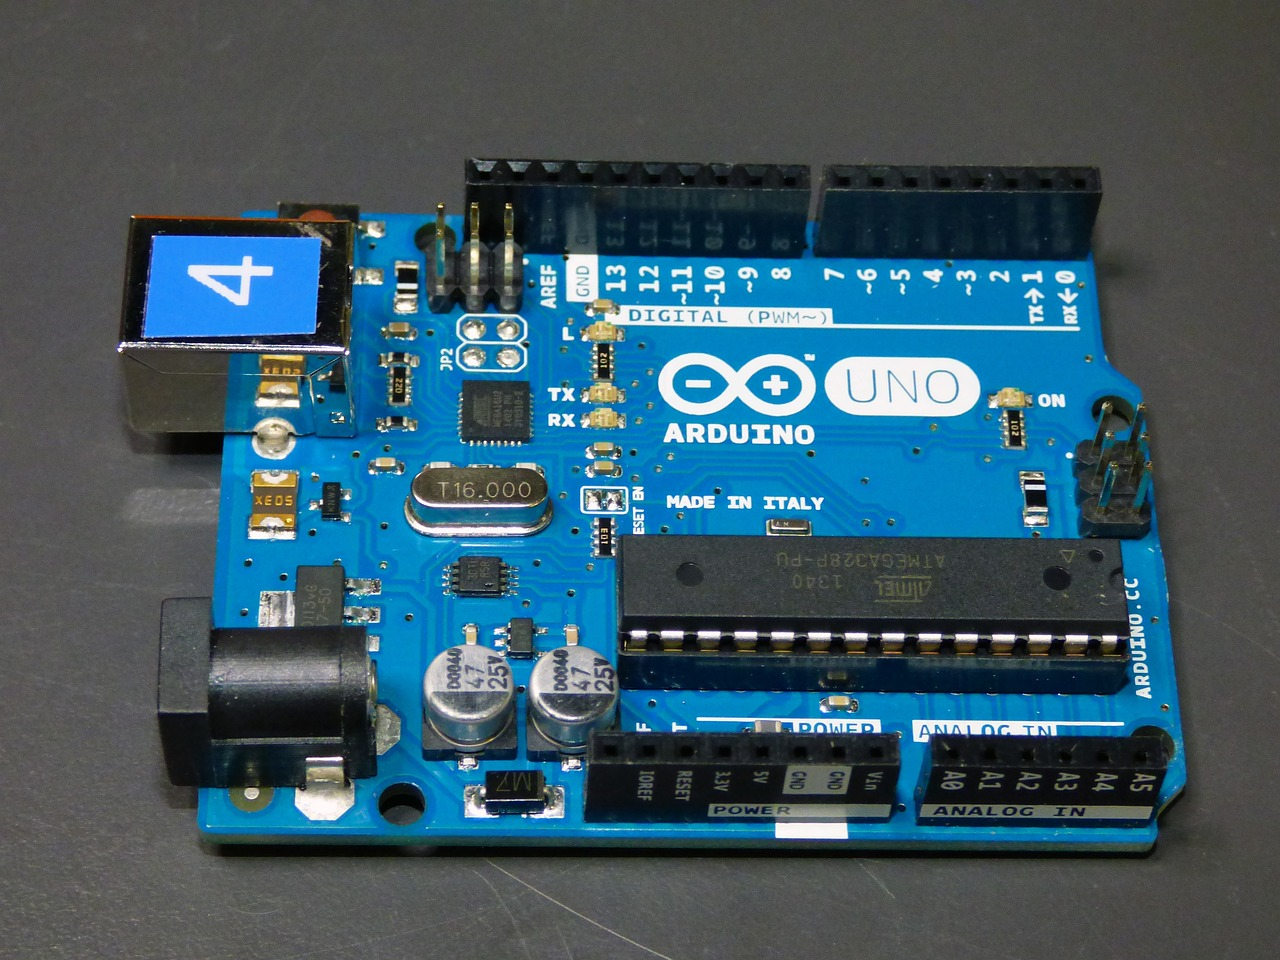
\includegraphics[width=1.9cm]{assets/Pixabay_Arduino_integrated-circuit-441289_1280.jpg} &
	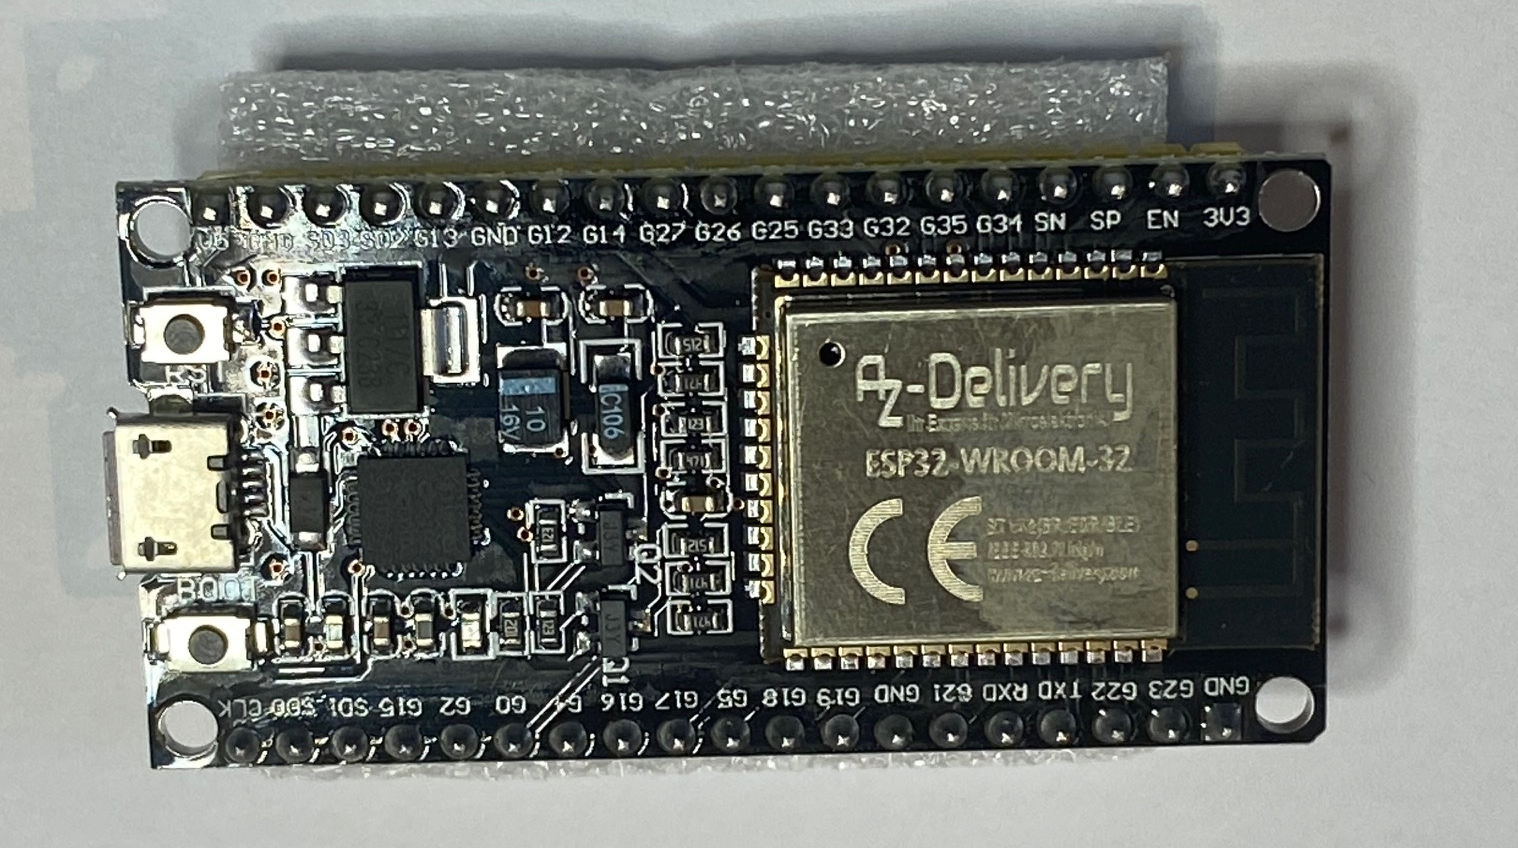
\includegraphics[width=1.9cm]{assets/ESP32.png} & 
	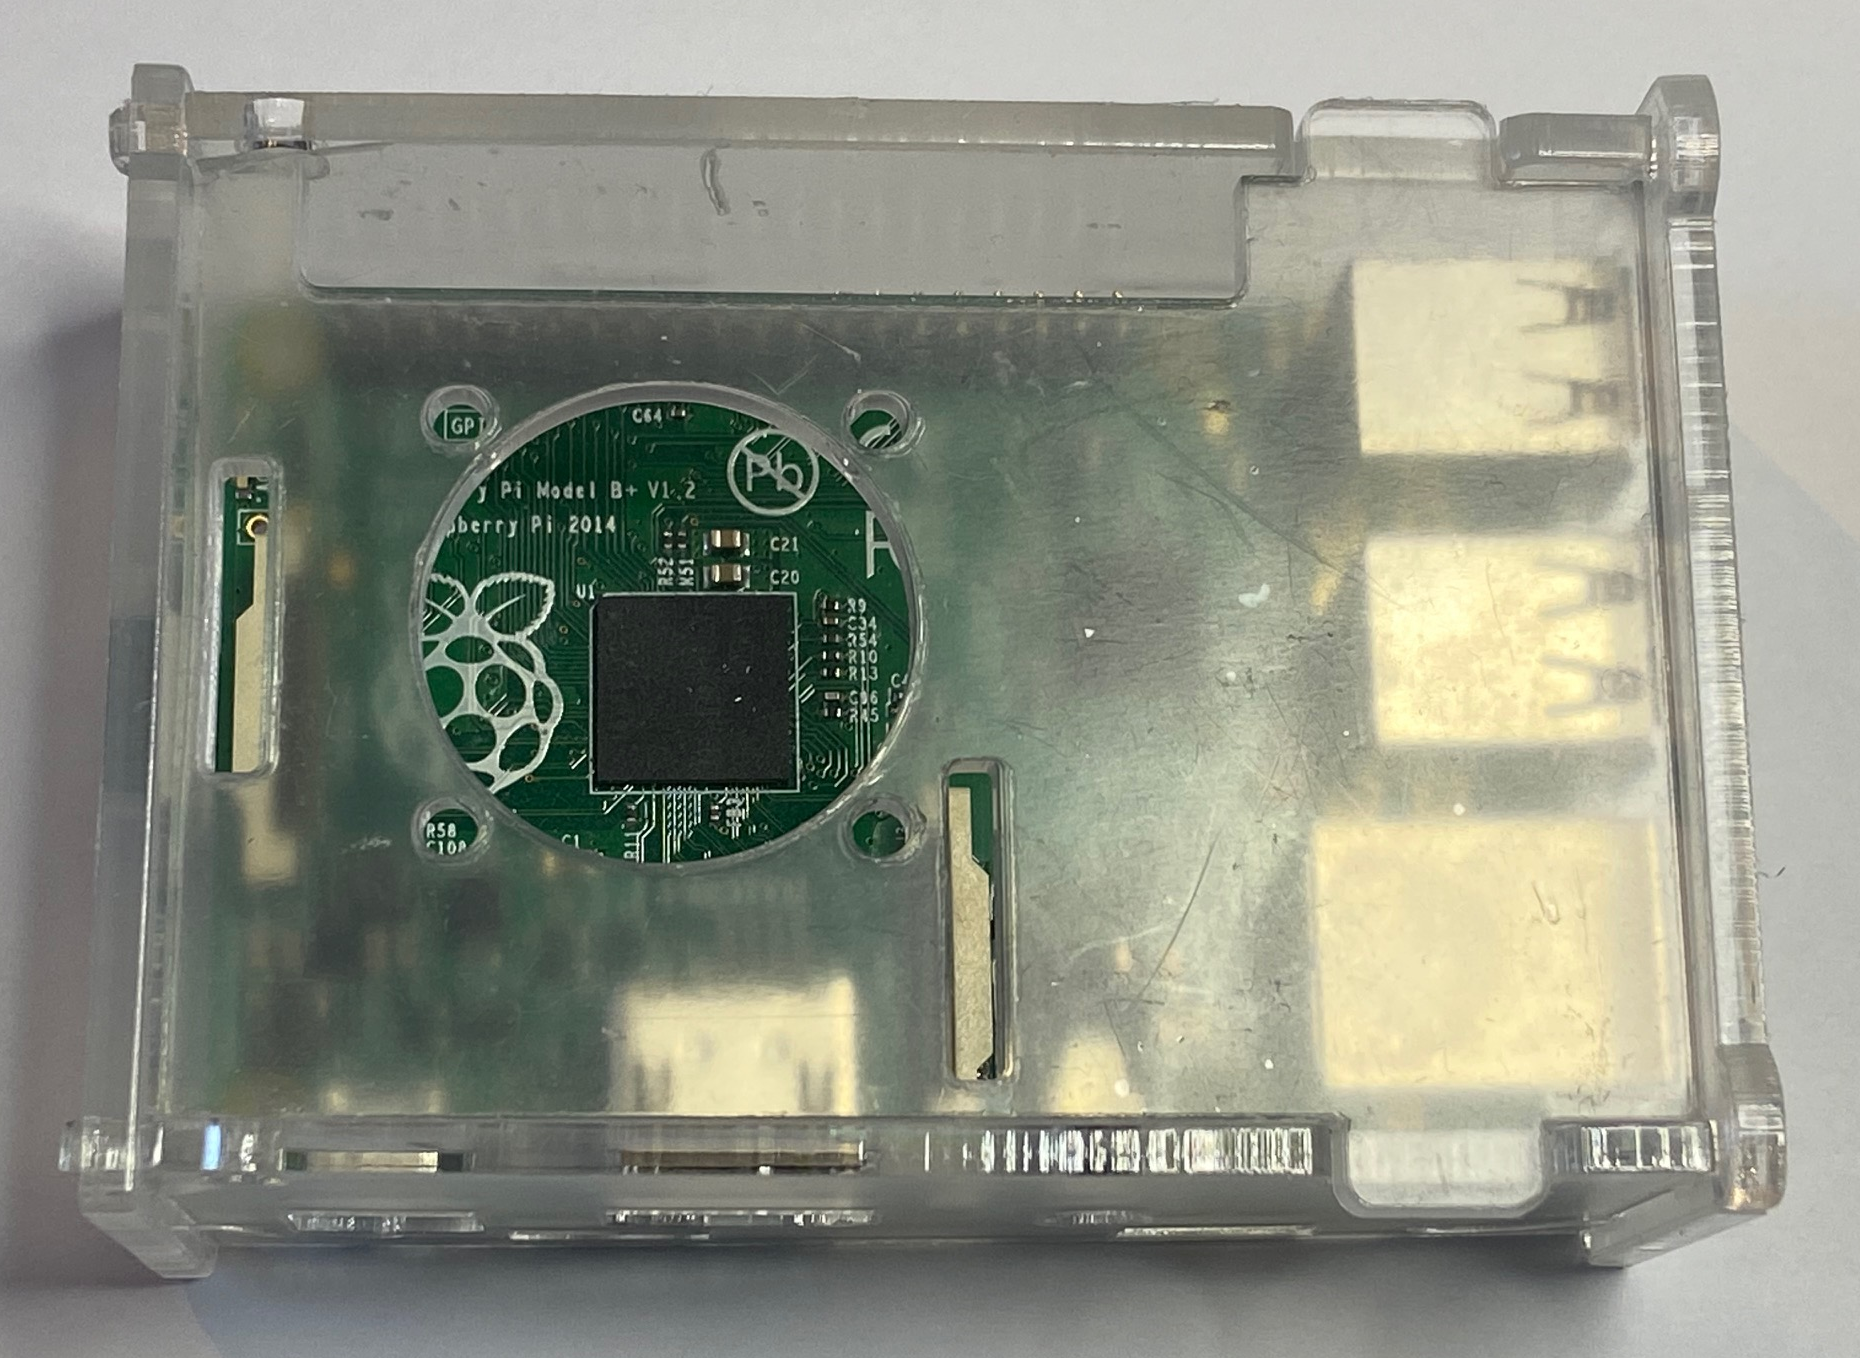
\includegraphics[width=1.9cm]{assets/Raspberry_Pi.png} \\
	&\textbf{Arduino} & \textbf{ESP32 FreeRTOS} & \textbf{SBC Linux} \\
	real-time & + &  + & - \\
	energy & + & o & - \\
	communication & - & o & + \\
	\end{tabular}
\end{frame}

\begin{frame}{What's the life-time of my project?}
	\begin{block}{What's the life-time?}
		Do I need to care about maintenance and updates?
	\end{block}
\end{frame}

\begin{frame}{What's the life-time of my project?}
	\begin{columns}[t]
    \column{0.33\textwidth}
        \centering
        \textbf{Experiment}
        \begin{itemize}
        		\item few months
        		\item no maintenance
        		\item some reusability
        \end{itemize}
    \column{0.33\textwidth}
        \centering
        \textbf{Media-Center}
        \begin{itemize}
        		\item some years
        		\item typical IT distribution maintenance
        		\item no reusability needed
        \end{itemize}
    \column{0.34\textwidth}
        \centering
        \textbf{Home Automation}
        \begin{itemize}
        		\item more than 15 years
        		\item \emph{maintenance and upgrades}
        		\item \emph{reusability for mid-term upgrade needed}
        \end{itemize}
    \end{columns}
\end{frame}

\section{Embedded Linux}

\begin{frame}{How to build an embedded Linux distribution?}
	\begin{block}{Topic}
		How to build a project specific embedded Linux distribution?
	\end{block}
\end{frame}

\begin{frame}{The "golden image" approach}
	\begin{itemize}
		\item starting from an existing Linux image, e.g. Raspberry Pi OS,
		\item install the required tools,
		\item and configure it,
		\item and freeze the image.
	\end{itemize}

	\begin{columns}[t]
    \column{0.5\textwidth}
        \centering
        \begin{itemize}
			\pro easy approach
			\pro maintained by used distribution
		\end{itemize}        
    \column{0.5\textwidth}
        \centering
        \begin{itemize}
        		\con solution and base distribution are mixed
        		\con no support for variants
        		\con lots of not needed software
        \end{itemize}
    \end{columns}
\end{frame}

\begin{frame}{The "from scratch" approach}
	\begin{itemize}
		\item using a built toolkit, e.g. Yocto or Buildroot
		\item which builds all packages from source
		\item using a project specific configuration and patches
	\end{itemize}

	\begin{columns}[t]
    \column{0.5\textwidth}
        \centering
        \begin{itemize}
        	\pro optimal system
        	\pro minimized resources
        	\pro reusable solution
        	\pro support for variants
        \end{itemize}
    \column{0.5\textwidth}
        \centering
        \begin{itemize}
        		\con learning curve
        		\con maintenance effort
        \end{itemize}
    \end{columns}
\end{frame}

\begin{frame}{The "remix" approach}
	\begin{itemize}
		\item use the packages from an existing distribution
		\item and create a solution-specific remix
		\item by reusing the exiting binary packages
		\item to build a custom image with customized configuration
	\end{itemize}

	\begin{columns}[t]
		\column{0.5\textwidth}
		\centering
		\begin{itemize}
			\pro low maintenance effort
			\pro smaller than "golden image"
			\pro reusable solution
			\pro support for variants
		\end{itemize}
		\column{0.5\textwidth}
		\centering
		\begin{itemize}
			\con learning curve
			\con limited optimization
		\end{itemize}
	\end{columns}
\end{frame}

\section{The source build toolkit}

\begin{frame}
	\begin{block}{Topic}
		How can I efficient build a customized embedded Linux distribution from scratch?
	\end{block}
\end{frame}

\begin{frame}{Tools for source builds}
	\begin{tabular}{c|ccc}
		& \textbf{Yocto} & \textbf{Buildroot}  \\
		\hline
		target & Embedded  & Embedded \\ 
		format & deb, rpm, arch & none \\
		cross toolchain & yes & yes \\
		flexibility & high & mid \\
	\end{tabular}
\end{frame}



\begin{frame}{Yocto}
	\begin{block}{Whats included?}
		Provides Metadata (recipes, configuration, data how things are built), BitBake (buildsystem) to build a custom embedded Linux distribution and a SDK. It also provides Poky as a reference distribution. Layer for many boards are available.
	\end{block}

	\begin{itemize}
		\item Builds packages and images based on recipes and configuration
		\item Metadata is using Bash and Python
		\item Docs: \href{https://docs.yoctoproject.org/}{docs.yoctoproject.org}
		\item Source: \url{git://git.yoctoproject.org/poky}
	\end{itemize}
\end{frame}

\begin{frame}{Buildroot}
	\begin{block}{Whats included?}
		Generate embedded Linux systems (Rootfs, Kernel, Bootloader, SDK)  based on a "Makefile collection" and configuration for a number of boards. Simpler then Yocto (easier, but less features)
	\end{block}

	\begin{itemize}
		\item Build components and images from source
		\item Style is based on Makefile and Kconfig 
		\item Docs: \href{https://buildroot.org/downloads/manual/manual.html}{buildroot.org/downloads/manual/manual.html}
		\item Source: \href{https://gitlab.com/buildroot.org/buildroot/}{gitlab.com/buildroot.org/buildroot/}
	\end{itemize}
\end{frame}

\section{Remixing a distribution}

\begin{frame}
	\begin{block}{Topic}
		How can I efficient build a remix embedded Linux distribution?
	\end{block}
\end{frame}

\begin{frame}{Tools for building a remix distribution}
	\begin{tabular}{c|ccc}
		& \textbf{Elbe} & \textbf{Debos} & \textbf{Kiwi-ng} \\
		\hline
		target & Embedded Image & Debian remix & Linux remix \\ 
		format & deb & deb & deb, rpm, arch \\
		cross toolchain & yes & no & no \\
		flexibility & mid & mid & low \\
	\end{tabular}
\end{frame}

\subsection{Kiwi-ng}

\begin{frame}{Kiwi-ng}
	\begin{block}{What's included?} 
		Kiwi-ng is a utility to build Linux system appliances. 
		An appliance is a ready to use image of an operating system including a pre-configured application for a specific use case. 
	\end{block}

	\begin{itemize}
		\item Supports all major package managers
		\item Image description using XML and config scripts
		\item Docs: \url{https://osinside.github.io/kiwi/}
		\item Source: \url{https://github.com/OSInside/kiwi}
	\end{itemize}
\end{frame}

\subsection{Debos}

\begin{frame}{Debos}
	\begin{block}{What's included?} 
		debos is a tool to make the creation of various Debian-based OS images simpler. While most other tools focus on specific use-cases, debos is more meant as a tool-chain to make common actions trivial while providing enough rope to do whatever tweaking that might be required behind the scene.
	\end{block}
	
	\begin{itemize}
		\item Supports only Debian packages
		\item Image description using YAML
		\item Docs: \url{https://pkg.go.dev/github.com/go-debos/debos}
		\item Source: \url{https://github.com/go-debos/debos}
	\end{itemize}
\end{frame}

\subsection{Elbe}

\begin{frame}{Elbe}
	\begin{block}{What's included?} 
		Elbe is a Debian-based system to generate root filesystems for embedded devices.
	\end{block}

	\begin{itemize}
		\item Supports only Debian packages
		\item Image description using XML
		\item Docs: \url{https://elbe-rfs.org/docs/sphinx}
		\item Source: \url{https://github.com/Linutronix/elbe}
	\end{itemize}
\end{frame}

\section{Minimal image}

\begin{frame}{Which tool should I use?}
	\begin{block}{Topic}
		What is the right tool for my project?
	\end{block}
\end{frame}

\begin{frame}{Which tool should I use?}
	\begin{itemize}
		\item Minimal image to compare the tools:
		\begin{itemize}
			\item QEMU target
			\item Systemd as init manager
			\item OpenSSH server as service
		\end{itemize}
	\end{itemize}
\end{frame}

\begin{frame}{Comparison of different tools}
	\begin{tabular}{c|ccccc}
		& \textbf{Build} & \textbf{Startup} & \textbf{Size} & \textbf{Processes} & \textbf{Packages} \\
		\hline
		Yocto(systemd) & 19:50 & ~7 s & 143 MB & 70 & - \\
 		Yocto & 19:59 & ~2.3 s & 10 MB & 42 & - \\ 
		Buildroot & 23:35 & ~3 s & 132 MB & 45 & - \\
		\hline
		Debos & 6:30 & ~14s & 701 MB & 64 & 143 \\
		Elbe & 7:19 & ~14s & 872 MB & 64 & 143 \\
		Kiwi-ng & 31:14 & ~14s & 691 MB & 63 & 143 \\
		\hline
		RPi OS & & ~16s & 1.7 GB & 151 & 597 \\
	\end{tabular}
\end{frame}

\section{Example project}

\begin{frame}{The coffee machine}
	The example project:
	\begin{itemize}
		\item Raspberry Pi 4 as target platform
		\item Systemd as init manager
		\item QT6 coffee demo as example application
		\item Requirements:
		\begin{itemize}
			\item The app shall start automatically in fullscreen mode
			\item The app shall own the graphics device (no window manager)
			\item The image shall only contain the minimal necessary dependencies (minimize maintenance and attack surface)
			\item For development, login with SSH shall be supported.
		\end{itemize}
	\end{itemize}
\end{frame}

\begin{frame}{The coffee machine}
	\begin{tabular}{cc}
		\href{https://github.com/qt/qtdoc/tree/v6.4.2/examples/demos/coffee}{QT 6.4.2} &
		\href{https://github.com/qt/qtdoc/tree/v6.6.2/examples/demos/coffee}{QT 6.6.2} \\
		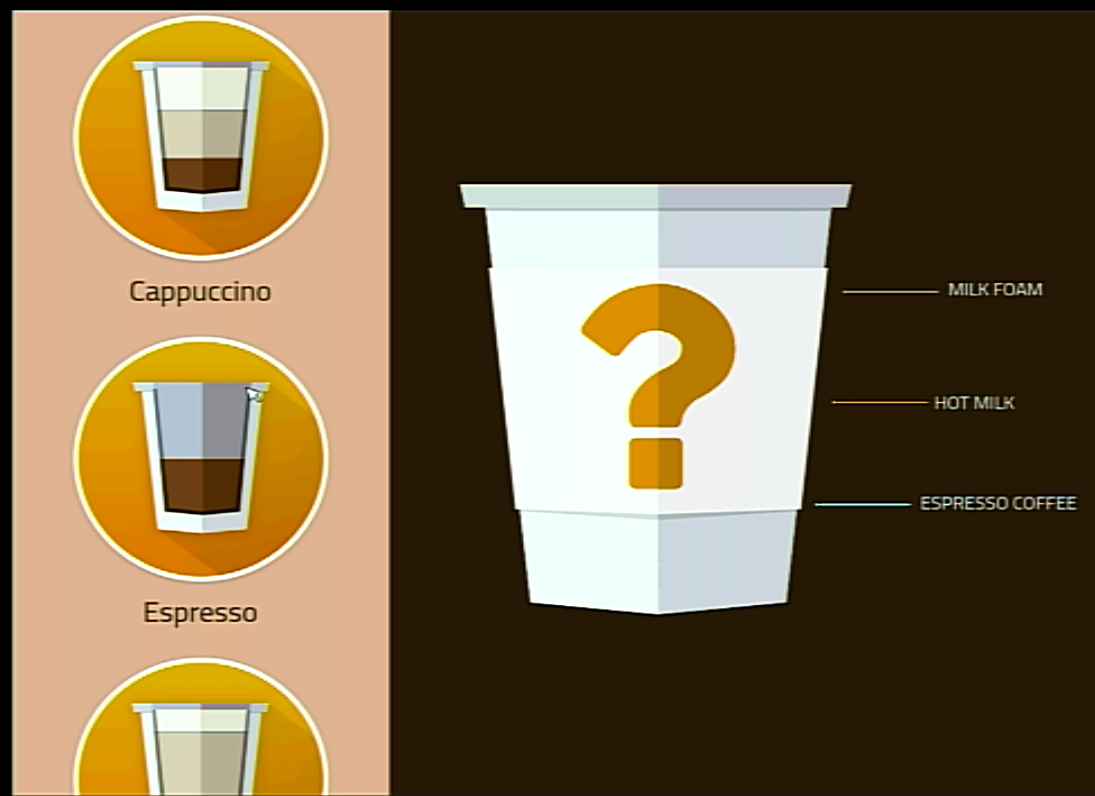
\includegraphics[width=5cm]{assets/Screenshot_Coffee_QT6.4.2.png} &
		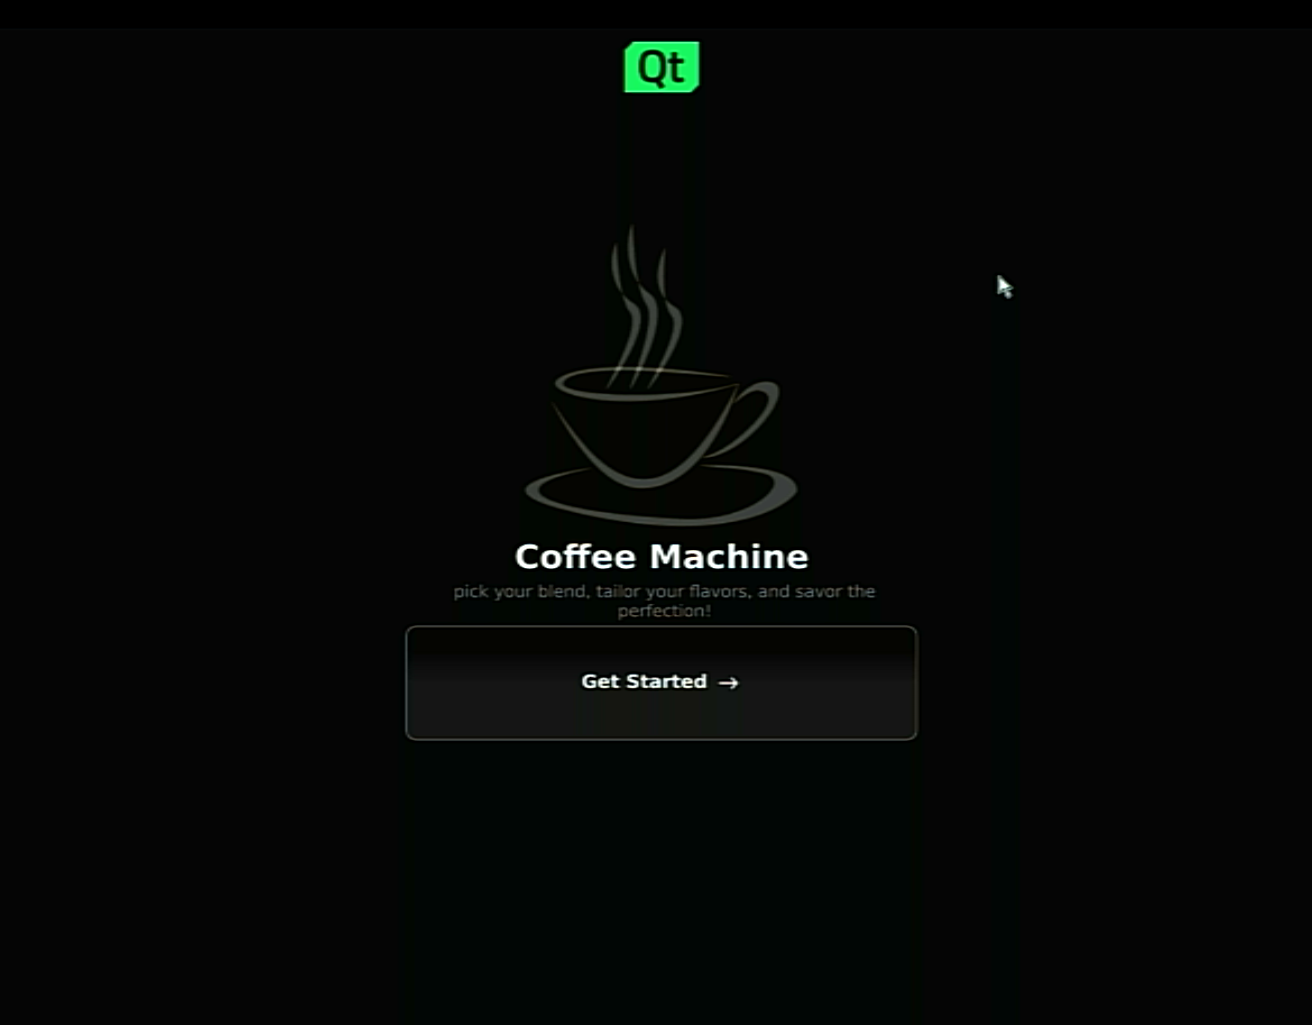
\includegraphics[width=5cm]{assets/Screenshot_Coffee_QT6.6.2.png} \\
	\end{tabular}
\end{frame}

\subsection{Coffee machine with Yocto}

\begin{frame}{How to realize this project with Yocto?}
	\begin{block}{How to do?}
		How to implement the coffee machine project with Yocto?
	\end{block}
\end{frame}


\begin{frame}{How to realize this project with Yocto?}
	\begin{block}{How to do?}
		How to implement the coffee machine project with Yocto?
	\end{block}
	You can find many layers for QT with yocto. One can follow
	\href{https://code.qt.io/cgit/yocto/meta-boot2qt.git/tree/README.md}{boot2qt} for the complete QT demo,
	but we will create a tailored image with meta-qt6. Find the code for this example at
	\href{https://github.com/tomirgang/eh21_maintainable_linux/tree/main/examples/yocto_advance/qt}{Github}.
\end{frame}

\begin{frame}{Step 1: Create coffee layer}
	First let us create a layer where our app and image can be implemented:
	\begin{itemize}
		\item Create an own layer for this work\\
			\emph{bitbake-layers create-layer ../meta-coffee}
		\item Add needed build dependencies\\
			\emph{LAYERDEPENDS\_meta-coffee = "core qt6-layer"}
		\item Add the layer to the conf\\
			\emph{bitbake-layers add-layer ../meta-coffee}
	\end{itemize}
	This should give you a folder meta-coffee where you can start implementing
	the coffee package and image.
\end{frame}

\begin{frame}{Step 2: Seperate the coffee app}
	Now let us adapt the existing package qtdoc from meta-qt6 to add a package
	containing only the wanted app:
	\begin{itemize}
		\item Create a qtdoc\_git.bbappend file for qtdoc in\\
			\emph{meta-coffee\/recipes-qt\/qt6}
		\item Create the qtdoc-coffee package\\
			\emph{PACKAGE\_BEFORE\_PN =+ "qtdoc-coffee"}	
		\item And add relevant files for the app\\
			\emph{PACKAGES =+ "qtdoc-coffee" \\
				  FILES:qtdoc-coffee = "\$\{QT6\_INSTALL\_EXAMPLESDIR\}/demos/coffee \$\{systemd\_unitdir\}/system/"}
	\end{itemize}
	This should give you a \emph{qtdoc-coffee} package that you can include in an image.
\end{frame}


\begin{frame}{Step 3: Create the coffee image}
	Next we can include the qtdoc-coffe package to an image
	\begin{itemize}
		\item Create a minimal-coffee.bb file for it in \emph{meta-coffee\/recipes-core\/images} and add\\
			\emph{inherit core-image}
		\item Add qtdoc-coffee and dependcies\\
			\emph{IMAGE\_INSTALL += "weston qtimageformats qtsvg qtdoc-coffee"}	
	\end{itemize}
	This should give you a \emph{minimal-coffee} image already. In rhe source you will additionally
	see how to enable autlogin.
\end{frame}

\begin{frame}{Step 4: Add coffee systemd service}
	Now let us adapt the qtdoc bbappend further with a systemd service to start the app
	directly.
	\begin{itemize}
		\item In qtdoc\_git.bbappend add\\
			\emph{inherit systemd \\
				 SYSTEMD\_SERVICE\_\$\{PN\}-coffee = "coffee.service" \\
				 SRC\_URI:append = " file://coffee.service" \\
				 do\_install:append() ...}
		\item Create the service under \emph{meta-coffee/recipes-qt/qt6/qtdoc/coffee.service}\\
				\emph{...\\
					  ExecStart=/usr/share/examples/demos/coffee/coffeemachine\\
					  ...}
	\end{itemize}
	This should give you a  \emph{minimal-coffee} that starts your \emph{coffeemachine}.
\end{frame}

\subsection{Coffee machine with Elbe}

\begin{frame}{How to realize this project with Elbe?}
	\begin{block}{How to do?}
		How to implement the coffee machine project with Elbe?
	\end{block}
\end{frame}

\begin{frame}{How to realize this project with Elbe?}
	\begin{block}{Using the Debian Bookworm QT packages}
		How to implement the coffee machine project with Elbe using the QT 6.4.2 packages provided by Debian Bookworm?
	\end{block}

	You can find the code for this example on
	\href{https://github.com/tomirgang/eh21_maintainable_linux/tree/main/examples/elbe_advanced}{Github}.
\end{frame}


\begin{frame}{Step 1: Ensure we can build the app}
	First we should make sure we can build the app:
	\begin{itemize}
		\item Install the needed build dependencies:\\
			\emph{sudo apt install qt6-base-dev qt6-declarative-dev}
		\item Get the source code of the example app
		\item Create a build folder and build the app:
		\begin{itemize}
			\item cmake \emph{path-to/coffee}
			\item make
		\end{itemize}
	\end{itemize}
	This should give you a \emph{coffee} binary which you can run.
\end{frame}

\begin{frame}{Step 2: Package the app - Debian metadata}
	Next we should create a Debian package for our app.\\
	To do this, we need to generate Debian metadata for the app:
	\begin{itemize}
		\item Install the needed tools:\\
		\emph{sudo apt install dh-make pbuilder debootstrap devscripts}
		\item Set the needed Debian maintainer environment variables:
		\begin{itemize}
			\item \emph{export DEBFULLNAME="Thomas Irgang"}
			\item \emph{export DEBEMAIL="thomas@irgang.eu"}
		\end{itemize}
		\item Rename the app folder using the pattern: \emph{app name}-\emph{app version}
		\item Generate the Debian metadata:
		\begin{itemize}
			\item Inside the app folder, run:
			\item \emph{dh\_make -n -s --yes}
		\end{itemize}
	\end{itemize}
	This will generate a \emph{debian} sub-folder containing lot's of prepared package metadata.
\end{frame}

\begin{frame}{Step 3: Package the app - fine-tune metadata}
	Now we need to fine-tune the generated metadata:
	\begin{itemize}
		\item Add the build dependencies:
		\begin{itemize}
			\item \emph{qt6-base-dev}
			\item \emph{qt6-declarative-dev}
		\end{itemize}
		\item During the package build, shared library dependencies will be filled automatically by \emph{shlibs}, but we need to add manually the dynamic loaded libraries:
		\begin{itemize}
			\item \emph{qml6-module-qtquick}
			\item \emph{qml6-module-qtquick-controls}
			\item \emph{qml6-module-qtquick-layouts}
			\item \emph{qml6-module-qtquick-templates}
			\item \emph{qml6-module-qtquick-window}
			\item \emph{qml6-module-qtqml-workerscript}
		\end{itemize}
	\end{itemize}
\end{frame}

\begin{frame}{Step 4: Package the app - configure pbuilder}
	Our image is based on Debian Bookwork. Configure pbuilder:
	\begin{itemize}
		\item Create \emph{.pbuilderrc}:
	\end{itemize}
	
	\small{\emph{echo "DISTRIBUTION=bookworm" $>>$ ~/.pbuilderrc} \\
	\emph{echo "MIRRORSITE=http://ftp.de.debian.org/debian" $>>$ ~/.pbuilderrc}}
	
	\begin{itemize}
		\item For cross-compilation support, we need to enable the apt dependency resolution:
	\end{itemize}
	\small{\emph{echo 'PBUILDERSATISFYDEPENDSCMD="/usr/lib/pbuilder/pbuilder-satisfydepends-apt"' $>>$ ~/.pbuilderrc}}
\end{frame}

\begin{frame}{Step 5: Package the app - build the package}
	Now we can build the app:
	\begin{itemize}
		\item Run \emph{pdebuild} in the folder containing the coffee app: \\ \emph{pdebuild -- --host-arch arm64}
	\end{itemize}
	This will generate a \emph{coffee\_6.4.2\_arm64.deb} in \emph{/var/cache/pbuilder/result}.
\end{frame}

\begin{frame}{Step 6: Install the app}
	\begin{itemize}
		\item Add app to image description: \emph{$<$pkg variant="app"$>$coffee$<$/pkg$>$}
		\item Build image with app:
		\small{\begin{itemize}
			\item \emph{elbe control create\_project $>$ my.prj}
			\item \emph{export PRJ=\$(cat my.prj)}
			\item \emph{elbe preprocess --variant app rpi-image/aarch64\_rpi4.xml}
			\item \emph{elbe control set\_xml \$PRJ preprocess.xml}
			\item \emph{elbe prjrepo upload\_pkg \$PRJ /var/cache/pbuilder/result/coffee\_6.4.2\_arm64.deb}
			\item \emph{elbe control build \$PRJ}
			\item wait for build finishing and download results.
		\end{itemize}}
	\end{itemize}
\end{frame}

\begin{frame}{Step 7: Auto-start the app}
	The final step is to automatically run the app on system startup.
	\begin{itemize}
		\item Create a systemd unit file to run the binary.
		\href{https://github.com/tomirgang/eh21_maintainable_linux/blob/main/examples/elbe_advanced/image/rpi-image/overlays/systemd/etc/systemd/system/coffee.service}{Github}
		\item Enable the new service using a \emph{finetuning} command:
		\begin{itemize}
			\item \emph{$<$command variant="app"$>$systemctl enable coffee$<$/command$>$}
		\end{itemize}
		\item Disable the getty on the HDMI tty:
		\begin{itemize}
			\item \emph{$<$command variant="app"$>$systemctl mask getty@tty1$<$/command$>$}
			\item \emph{$<$command variant="app"$>$systemctl disable getty@tty1$<$/command$>$}
		\end{itemize}
	\end{itemize}
\end{frame}

\section{The End}

\begin{frame}{The End}
	\begin{block}{Any questions?}
		We hope you enjoyed the talk.
		Your questions are now welcome!
	\end{block}
\end{frame}

\section{How to build a Raspberry Pi image?}


\begin{frame}{Yocto: Raspberry Pi image}
	\begin{itemize}
		\item Source: \href{https://git.yoctoproject.org/poky}{poky}, \href{https://git.yoctoproject.org/meta-raspberrypi/}{bsp}
		\item based on Poky
		\item Steps:
		\begin{itemize}
			\item install kas: pip3 install kas
			\item get kas.yml
			\item run kas build
			\item copy image to SD card
		\end{itemize}
		\item more details on \href{https://github.com/tomirgang/eh21_maintainable_linux/tree/main/examples/first_build_rpi4/yocto}{Github}
	\end{itemize}
\end{frame}


\begin{frame}{Buildroot: Raspberry Pi image}
	\begin{itemize}
		\item Source: \href{https://gitlab.com/buildroot.org/buildroot/}{GitLab}
		\item Steps:
		\begin{itemize}
			\item install \href{https://buildroot.org/downloads/manual/manual.html\#requirement}{dependencies}
			\item make raspberrypi4\_64\_defconfig
			\item make
			\item copy image to SD card
		\end{itemize}
		\item more details on \href{https://github.com/tomirgang/eh21_maintainable_linux/tree/main/examples/first_build_rpi4/buildroot}{Github}
	\end{itemize}
\end{frame}

\begin{frame}{Kiwi-ng: Raspberry Pi image}
	\begin{itemize}
		\item Source: \href{https://github.com/OSInside/kiwi-descriptions/tree/main/ubuntu/aarch64/ubuntu-jammy-rpi}{Github}
		\item based on Ubuntu Jammy
		\item Steps:
		\begin{itemize}
			\item install \url{https://pypi.org/project/kiwi/}
			\item install \url{https://pypi.org/project/kiwi-boxed-plugin/}
			\item get image description
			\item run image build
			\item copy image to SD card
		\end{itemize}
		\item more details on \href{https://github.com/tomirgang/eh21_maintainable_linux/tree/main/examples/first_build_rpi4/kiwi-ng}{Github}
	\end{itemize}
\end{frame}


\begin{frame}{Debos: Raspberry Pi image}
	\begin{itemize}
		\item Source: \href{https://github.com/go-debos/debos-recipes/tree/main/rpi64}{Github}
		\item based on Debian Bullseye
		\item Steps:
		\begin{itemize}
			\item Debian: install debos packages
			\item run image build
			\item copy image to SD card
		\end{itemize}
		\item more details on \href{https://github.com/tomirgang/eh21_maintainable_linux/tree/main/examples/first_build_rpi4/debos}{Github}
	\end{itemize}
\end{frame}


\begin{frame}{Elbe: Raspberry Pi image}
	\begin{itemize}
		\item Based on \href{https://github.com/Linutronix/elbe/blob/master/examples/arm64-qemu-virt.xml}{example arm64-qemu-virt}
		\item Steps:
		\begin{itemize}
			\item Debian: install elbe package
			\item prepare the initvm
			\item run the image build
			\item copy image to SD card
		\end{itemize}
		\item more details on \href{https://github.com/tomirgang/eh21_maintainable_linux/tree/main/examples/first_build_rpi4/elbe}{Github}
	\end{itemize}
\end{frame}


\end{document}
